%2multibyte Version: 5.50.0.2960 CodePage: 65001
% !TeX root = ./Slides_Lez_14_Programmazione_Stocastica_I.tex
% ------------------------------------------------------------
% Slides Lezione 14 - Programmazione lineare stocastica I
% Programmazione stocastica a due stadi
% Progetto MQF - Metodi Quantitativi per la Finanza
% Macro matematiche ufficiali del progetto MQF
% Coerenti con MQF_Notazione.tex
% Vocali accentate nella forma \`a, \`e, \'e, senza parentesi graffe
% ------------------------------------------------------------
% Fallback utile per compilazione esterna se qualche titolo resta scritto come \QTR.
% Scientific WorkPlace usa \QTR internamente; in Beamer \QTR{frametitle}{Titolo}
% deve espandersi in \frametitle{Titolo}.

\documentclass[handout]{beamer}%
\usepackage{mathpazo}
%\usepackage{hyperref}
\usepackage{multimedia}
\usepackage{amsmath}
\usepackage{amsfonts}
\usepackage{amssymb}
\usepackage{graphicx}%
\setcounter{MaxMatrixCols}{30}
%TCIDATA{OutputFilter=latex2.dll}
%TCIDATA{Version=5.50.0.2960}
%TCIDATA{Codepage=65001}
%TCIDATA{CSTFile=beamer.cst}
%TCIDATA{<META NAME="GraphicsSave" CONTENT="32">}
%TCIDATA{<META NAME="SaveForMode" CONTENT="2">}
%TCIDATA{BibliographyScheme=Manual}
%TCIDATA{<META NAME="DocumentShell" CONTENT="Other Documents\SW\Slides - Beamer">}
%BeginMSIPreambleData
\providecommand{\U}[1]{\protect\rule{.1in}{.1in}}
%EndMSIPreambleData
\newenvironment{stepenumerate}{\begin{enumerate}[<+->]}{\end{enumerate}}
\newenvironment{stepitemize}{\begin{itemize}[<+->]}{\end{itemize} }
\newenvironment{stepenumeratewithalert}{\begin{enumerate}[<+-| alert@+>]}{\end{enumerate}}
\newenvironment{stepitemizewithalert}{\begin{itemize}[<+-| alert@+>]}{\end{itemize} }
\usetheme{Madrid}
\providecommand{\R}{\mathbb{R}}
\providecommand{\N}{\mathbb{N}}
\providecommand{\E}{\mathbb{E}}
\providecommand{\Prob}{\mathbb{P}}
\providecommand{\Q}{\mathbb{Q}}
\providecommand{\F}{\mathcal{F}}
\providecommand{\B}{\mathcal{B}}
\providecommand{\G}{\mathcal{G}}
\providecommand{\Var}{\operatorname{Var}}
\providecommand{\Cov}{\operatorname{Cov}}
\providecommand{\VaR}{\operatorname{VaR}}
\providecommand{\CVaR}{\operatorname{CVaR}}
\providecommand{\argmin}{\operatorname*{arg\,min}}
\providecommand{\argmax}{\operatorname*{arg\,max}}
\providecommand{\EVPI}{\operatorname{EVPI}}
\providecommand{\VSS}{\operatorname{VSS}}
\providecommand{\QTR}[2]{\csname #1\endcsname{#2}}
%BeginMSIPreambleData
\ifx\pdfoutput\relax\let\pdfoutput=\undefined\fi
\newcount\msipdfoutput
\ifx\pdfoutput\undefined\else
\ifcase\pdfoutput\else
\msipdfoutput=1
\ifx\paperwidth\undefined\else
\ifdim\paperheight=0pt\relax\else\pdfpageheight\paperheight\fi
\ifdim\paperwidth=0pt\relax\else\pdfpagewidth\paperwidth\fi
\fi\fi\fi
%EndMSIPreambleData


\title[Programmazione Stocastica I]{Lezione 14 -- Programmazione lineare stocastica I: programmazione
stocastica a due stadi}
\subtitle{Metodi Quantitativi per la Finanza}
\author[P. Falbo, C. Pelizzari]{{\LARGE Paolo Falbo, Cristian Pelizzari}}
\institute[]{{\large Dipartimento di Economia e Management}}
\date[]{}
\titlegraphic{

\includegraphics[width=3.3cm]{../graphics/logo-Unibs-esteso.png}
}

\begin{document}
\maketitle

%****************************************

\section{Apertura}

\subsection{L'ALM deterministico}%

%TCIMACRO{\TeXButton{BeginFrame}{\begin{frame}}}%
%BeginExpansion
\begin{frame}%
%EndExpansion

\QTR{frametitle}{Dove eravamo: l'ALM deterministico}

%TCIMACRO{\TeXButton{Transparency}{\setbeamercovered{transparent=20}}}%
%BeginExpansion
\setbeamercovered{transparent=20}%
%EndExpansion

Nel modello ALM del Capitolo~12 i coefficienti futuri sono trattati come
\textbf{noti} al momento della decisione iniziale.

\medskip

\begin{stepitemize}
\item Cash flow $a_{tj}$, fabbisogni $d_t$, tassi $r_t^{g}$ e $r_t^{u}$,
capacit\`a di funding $\bar u_t$: tutta la traiettoria \`e un dato.

\item Composizione dell'attivo $x$, giacenze $g_t$ e funding $u_t$ vengono
quindi determinati \textbf{congiuntamente} al tempo $0$.
\end{stepitemize}

\medskip

\begin{block}{Un'ipotesi molto forte}
{\small Deterministico non significa costante: significa \textbf{noto in
anticipo}. Il piano fissa oggi anche il funding che verr\`a raccolto fra tre
periodi.}
\end{block}

%TCIMACRO{\TeXButton{Transition: Box Out}{\transboxout}}%
%BeginExpansion
\transboxout%
%EndExpansion
%TCIMACRO{\TeXButton{EndFrame}{\end{frame}}}%
%BeginExpansion
\end{frame}%
%EndExpansion

%****************************************

\subsection{La domanda della lezione}%

%TCIMACRO{\TeXButton{BeginFrame}{\begin{frame}}}%
%BeginExpansion
\begin{frame}%
%EndExpansion

\QTR{frametitle}{La domanda della lezione}

%TCIMACRO{\TeXButton{Transparency}{\setbeamercovered{transparent=20}}}%
%BeginExpansion
\setbeamercovered{transparent=20}%
%EndExpansion

Questa lezione rimuove l'ipotesi: una parte delle decisioni va assunta
\textbf{prima} di conoscere il futuro, altre \textbf{dopo} la rivelazione
dell'incertezza.

\medskip

\begin{block}{Domanda guida}
{\small Come si decide oggi quando il futuro pu\`o evolvere in modi diversi e
le possibilit\`a di reagire domani dipendono dalle scelte fatte oggi?}
\end{block}

\medskip

\[
\boxed{
\text{un unico futuro noto}
\qquad\longrightarrow\qquad
\text{pi\`u futuri possibili}
}
\]

\medskip

\begin{center}
{\small La distinzione essenziale \`e tra dimensione temporale e incertezza:
un problema pu\`o essere multiperiodale senza essere stocastico.}
\end{center}

%TCIMACRO{\TeXButton{Transition: Box Out}{\transboxout}}%
%BeginExpansion
\transboxout%
%EndExpansion
%TCIMACRO{\TeXButton{EndFrame}{\end{frame}}}%
%BeginExpansion
\end{frame}%
%EndExpansion

%****************************************

\subsection{Percorso della lezione}%

%TCIMACRO{\TeXButton{BeginFrame}{\begin{frame}}}%
%BeginExpansion
\begin{frame}%
%EndExpansion

\QTR{frametitle}{Percorso e obiettivi}

%TCIMACRO{\TeXButton{Transparency}{\setbeamercovered{transparent=20}}}%
%BeginExpansion
\setbeamercovered{transparent=20}%
%EndExpansion

{\small
\[
\begin{aligned}
&\text{modello probabilistico}
\longrightarrow
\text{scenari}
\longrightarrow
\text{ricorso}\\
&\hspace{2.0cm}
\longrightarrow
\text{programma stocastico}
\longrightarrow
\text{forma estesa}
\end{aligned}
\]
}

\begin{stepenumerate}
\item [1.] Distinguere \textbf{periodi temporali} e \textbf{stadi
decisionali}.

\item [2.] Rappresentare l'incertezza mediante \textbf{scenari} e
probabilit\`a, anche generati da una catena di Markov.

\item [3.] Definire e interpretare la \textbf{funzione di ricorso}.

\item [4.] Formulare il \textbf{programma lineare stocastico a due stadi}.

\item [5.] Costruire la \textbf{forma estesa}, riconoscendo il ruolo della non
anticipativit\`a.
\end{stepenumerate}

\medskip

Tre esercizi in aula accompagnano il percorso.

%TCIMACRO{\TeXButton{Transition: Box Out}{\transboxout}}%
%BeginExpansion
\transboxout%
%EndExpansion
%TCIMACRO{\TeXButton{EndFrame}{\end{frame}}}%
%BeginExpansion
\end{frame}%
%EndExpansion

%****************************************

\section{Incertezza e struttura informativa}

\subsection{Dati aleatori}%

%TCIMACRO{\TeXButton{BeginFrame}{\begin{frame}}}%
%BeginExpansion
\begin{frame}%
%EndExpansion

\QTR{frametitle}{Dalla traiettoria nota ai dati aleatori}

%TCIMACRO{\TeXButton{Transparency}{\setbeamercovered{transparent=20}}}%
%BeginExpansion
\setbeamercovered{transparent=20}%
%EndExpansion

\textbf{Caso deterministico}: alla data $t$ un vettore di dati fissati,
{\small
\[
\bar\xi_t=(\bar\xi_{t1},\ldots,\bar\xi_{tm})'\in\R^m,
\qquad
t\in\mathcal T.
\]
}
{\footnotesize La barra indica valori fissati nel problema, non valori attesi.}

\medskip

\textbf{Caso incerto}: gli stessi dati diventano vettori aleatori,
{\small
\[
\xi_t:(\Omega,\F)\longrightarrow(\R^m,\B(\R^m)),
\qquad
\xi=(\xi_1,\ldots,\xi_T).
\]
}

\begin{stepitemize}
\item Per ogni $\omega$, la successione $\xi_0(\omega),\ldots,\xi_T(\omega)$ \`e
una possibile traiettoria dei dati esogeni.

\item Nessuna ipotesi di indipendenza fra componenti o fra date: le
dipendenze appartengono alla legge congiunta del processo.

\item Caso SVB--ALM:
$\bar Z_t=(\bar R_t,\bar C_t,\bar F_t)\longrightarrow
Z_t=(Z_t^R,Z_t^C,Z_t^F)$.
\end{stepitemize}

%TCIMACRO{\TeXButton{Transition: Box Out}{\transboxout}}%
%BeginExpansion
\transboxout%
%EndExpansion
%TCIMACRO{\TeXButton{EndFrame}{\end{frame}}}%
%BeginExpansion
\end{frame}%
%EndExpansion

%****************************************

\subsection{Struttura a due stadi}%

%TCIMACRO{\TeXButton{BeginFrame}{\begin{frame}}}%
%BeginExpansion
\begin{frame}%
%EndExpansion

\QTR{frametitle}{Prima si decide, poi si osserva}

%TCIMACRO{\TeXButton{Transparency}{\setbeamercovered{transparent=20}}}%
%BeginExpansion
\setbeamercovered{transparent=20}%
%EndExpansion

\begin{center}
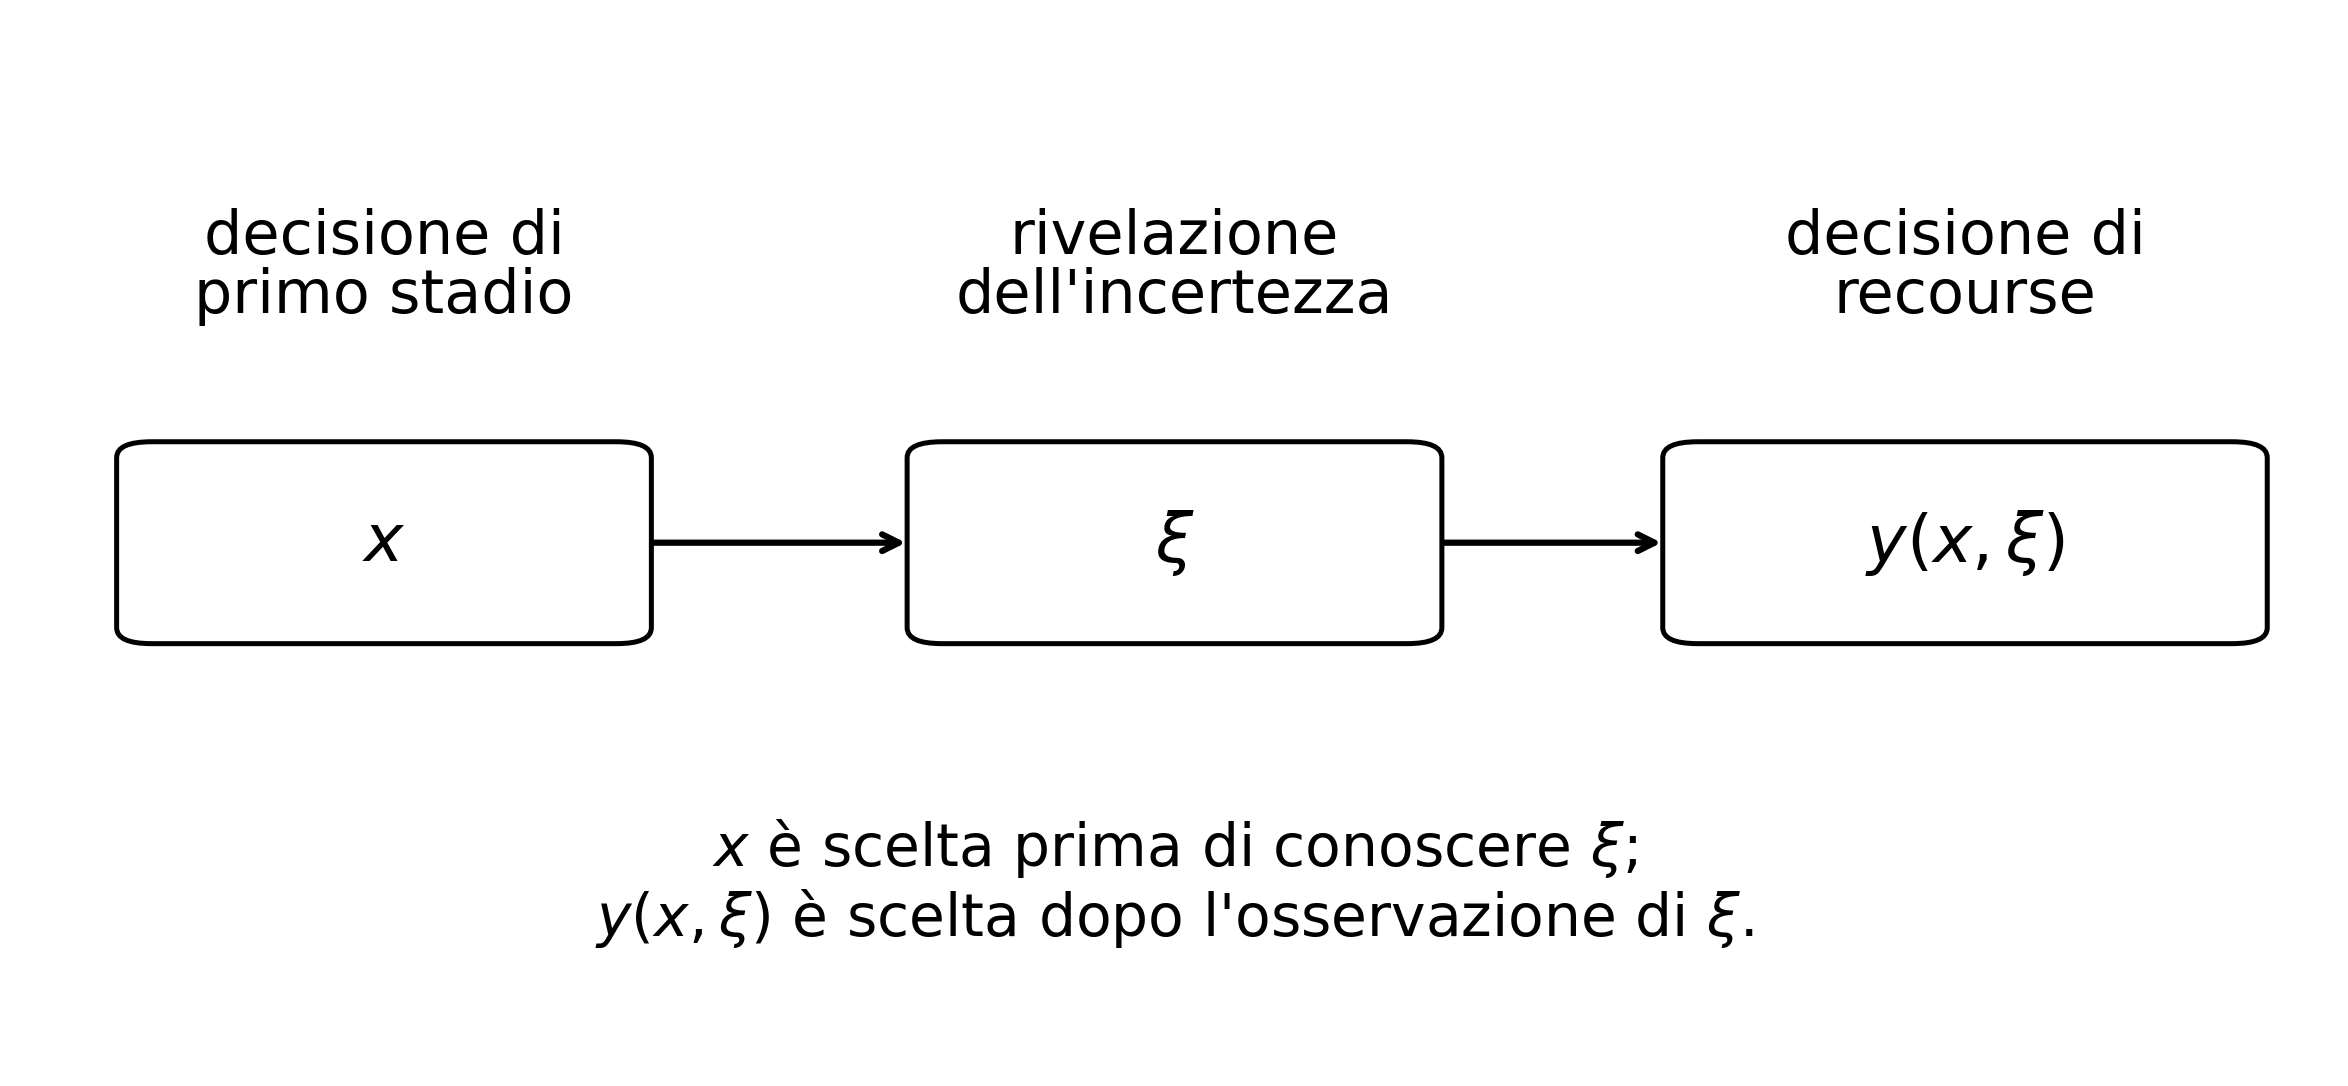
\includegraphics[width=0.70\textwidth]
{../graphics/Cap14_struttura_two_stage.png}
\end{center}

\vspace{-3mm}

\[
x
\longrightarrow
\xi
\longrightarrow
y(x,\xi)
\]

{\small
\begin{stepitemize}
\item La figura rappresenta una sequenza \textbf{informativa}, non una
successione di periodi temporali.

\item Il ricorso non annulla la decisione iniziale: reagisce alle condizioni
osservate \textbf{entro le possibilit\`a lasciate aperte} da $x$.
\end{stepitemize}
}

%TCIMACRO{\TeXButton{Transition: Box Out}{\transboxout}}%
%BeginExpansion
\transboxout%
%EndExpansion
%TCIMACRO{\TeXButton{EndFrame}{\end{frame}}}%
%BeginExpansion
\end{frame}%
%EndExpansion

%****************************************

\subsection{Stadi e periodi}%

%TCIMACRO{\TeXButton{BeginFrame}{\begin{frame}}}%
%BeginExpansion
\begin{frame}%
%EndExpansion

\QTR{frametitle}{Stadi decisionali e periodi temporali}

%TCIMACRO{\TeXButton{Transparency}{\setbeamercovered{transparent=20}}}%
%BeginExpansion
\setbeamercovered{transparent=20}%
%EndExpansion

\[
\text{numero dei periodi economici}
\qquad\neq\qquad
\text{numero degli stadi decisionali}
\]

\begin{stepitemize}
\item Un problema pu\`o svilupparsi lungo numerose date e restare a due stadi:
conta la posizione delle decisioni rispetto alla rivelazione
dell'incertezza.

\item Se $\xi$ riguarda pi\`u date, al secondo stadio l'intera realizzazione
rilevante \`e nota: i periodi contenuti nel ricorso condividono lo stesso
livello informativo.
\end{stepitemize}

\medskip

\textbf{Caso SVB--ALM}:
{\small
\[
x=(x_1,x_2,x_3,x_4)'
\longrightarrow
\xi
\longrightarrow
y(x,\xi)=(g_1,g_2,g_3,g_4,u_1,u_2,u_3)'.
\]
}

{\footnotesize Anche $u_1$ pu\`o dipendere dall'intera realizzazione di $\xi$:
\`e l'ipotesi informativa del modello a due stadi, non una propriet\`a
dell'ALM.}

%TCIMACRO{\TeXButton{Transition: Box Out}{\transboxout}}%
%BeginExpansion
\transboxout%
%EndExpansion
%TCIMACRO{\TeXButton{EndFrame}{\end{frame}}}%
%BeginExpansion
\end{frame}%
%EndExpansion

%****************************************

\section{Scenari}

\subsection{Rappresentazione a scenari}%

%TCIMACRO{\TeXButton{BeginFrame}{\begin{frame}}}%
%BeginExpansion
\begin{frame}%
%EndExpansion

\QTR{frametitle}{Rappresentare l'incertezza con scenari}

%TCIMACRO{\TeXButton{Transparency}{\setbeamercovered{transparent=20}}}%
%BeginExpansion
\setbeamercovered{transparent=20}%
%EndExpansion

\begin{center}
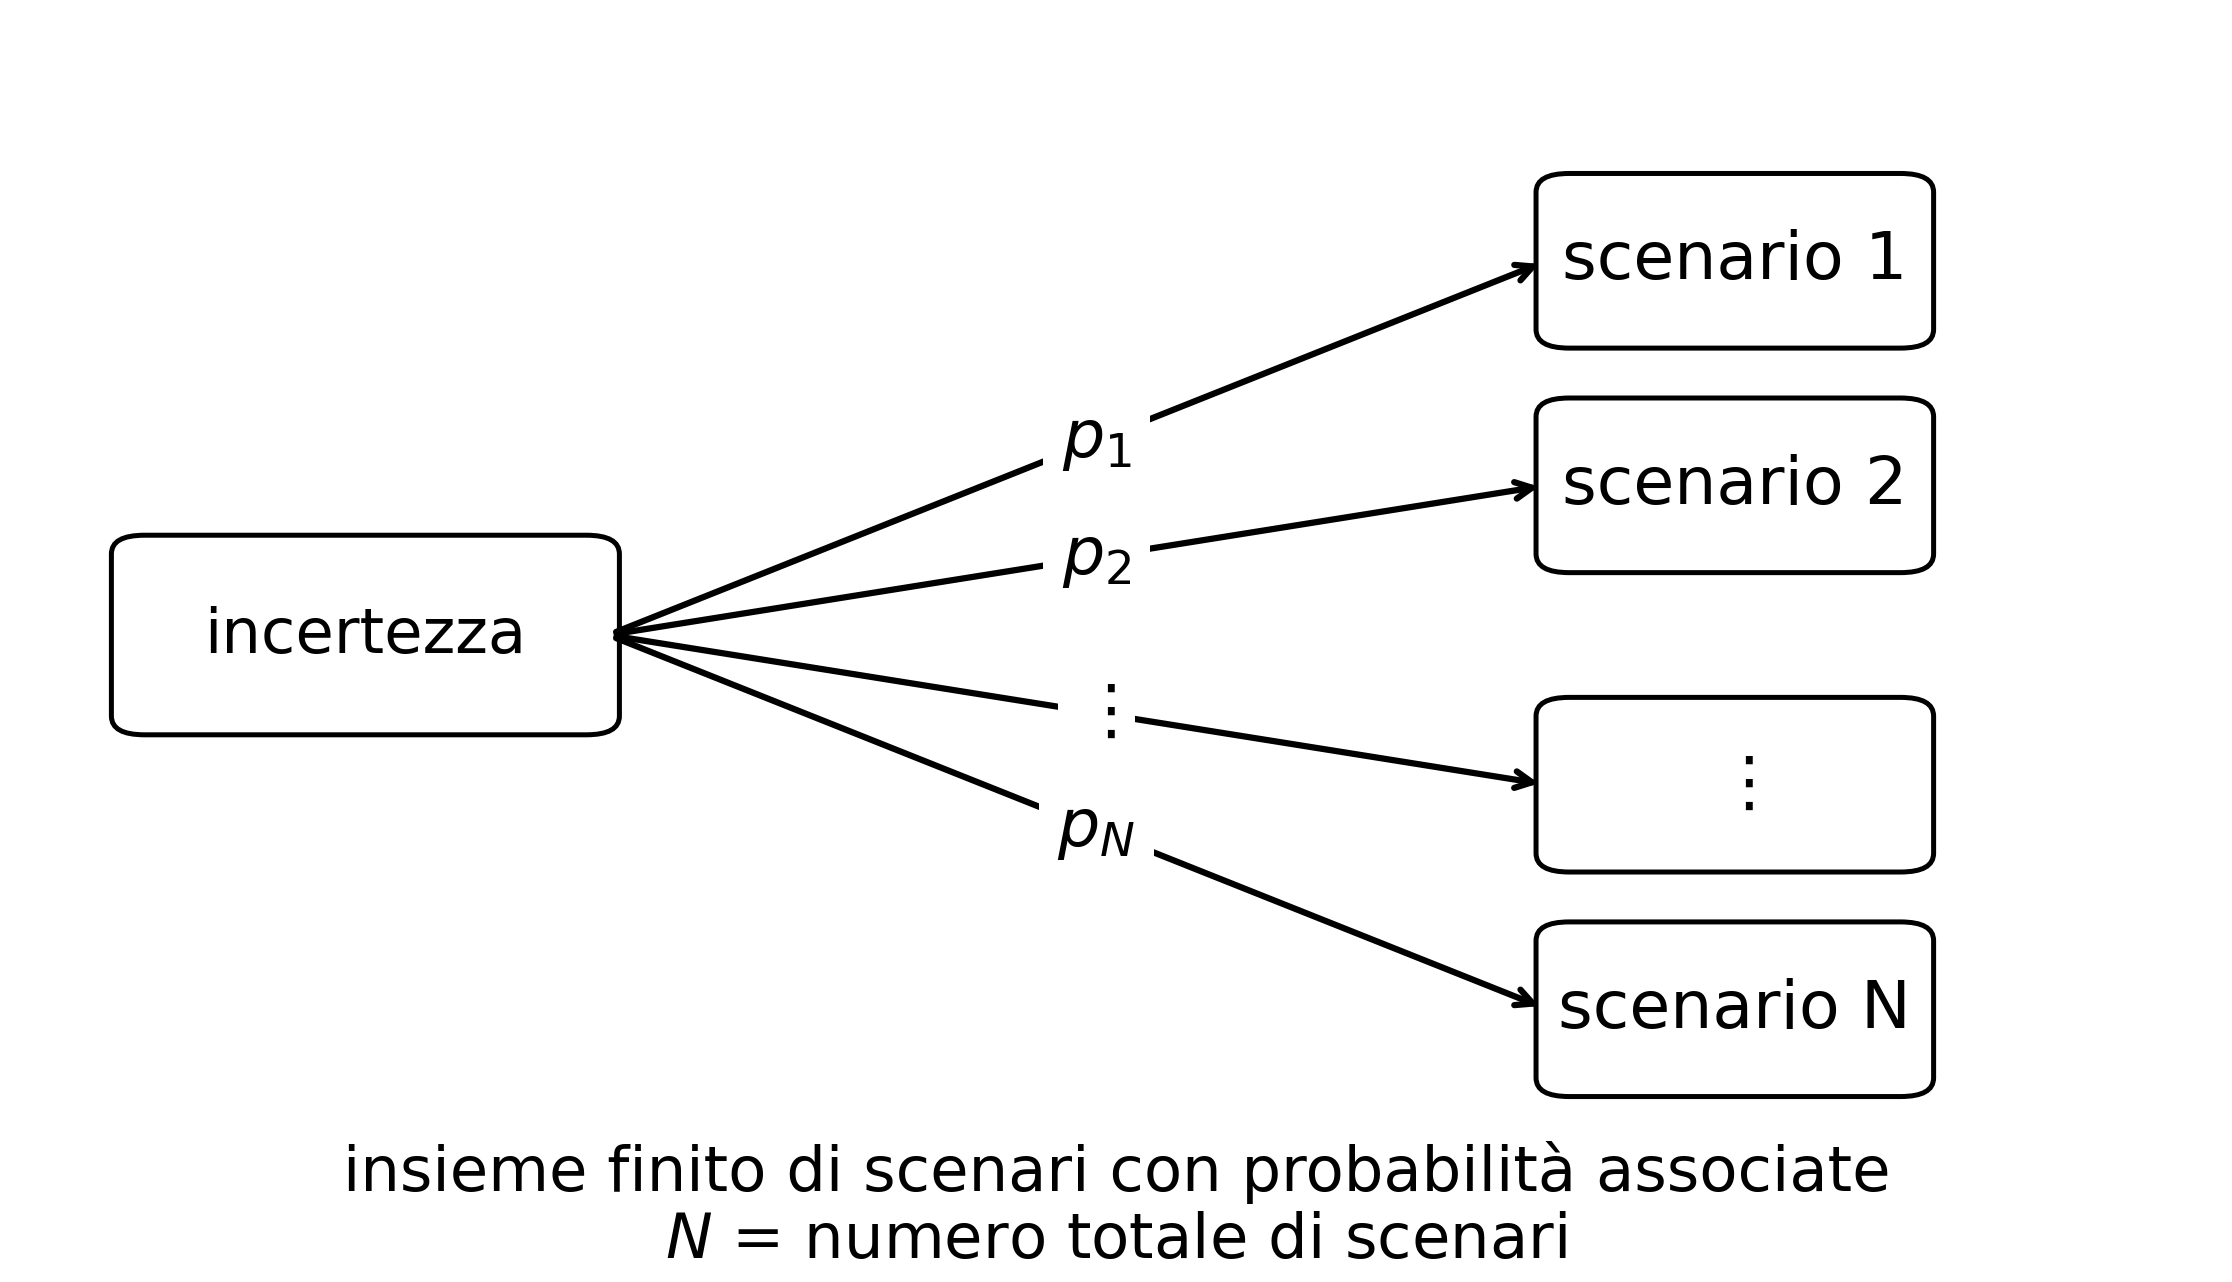
\includegraphics[width=0.52\textwidth]
{../graphics/Cap14_rappresentazione_scenari.png}
\end{center}

\vspace{-3mm}

{\small
\[
\left\{(\xi_s,p_s):s\in\mathcal S\right\},
\qquad
p_s\geq0,
\qquad
\sum_{s\in\mathcal S}p_s=1,
\qquad
\E[\varphi(\xi)]=\sum_{s\in\mathcal S}p_s\varphi(\xi_s).
\]
}

{\small
\begin{stepitemize}
\item Uguaglianza esatta se si includono tutti i valori di un supporto finito;
altrimenti approssimazione.

\item Con pi\`u date uno scenario \`e la traiettoria completa
$\xi_s=(\xi_1^s,\ldots,\xi_T^s)$, \textbf{non} lo stato a una singola data.
\end{stepitemize}
}

%TCIMACRO{\TeXButton{Transition: Box Out}{\transboxout}}%
%BeginExpansion
\transboxout%
%EndExpansion
%TCIMACRO{\TeXButton{EndFrame}{\end{frame}}}%
%BeginExpansion
\end{frame}%
%EndExpansion

%****************************************

\subsection{Costruzione degli scenari}%

%TCIMACRO{\TeXButton{BeginFrame}{\begin{frame}}}%
%BeginExpansion
\begin{frame}%
%EndExpansion

\QTR{frametitle}{Come si costruiscono gli scenari}

%TCIMACRO{\TeXButton{Transparency}{\setbeamercovered{transparent=20}}}%
%BeginExpansion
\setbeamercovered{transparent=20}%
%EndExpansion

\begin{stepitemize}
\item \textbf{Enumerazione esatta}: supporto finito e gestibile,
$p_s=\Prob(\xi=\xi_s)$, nessuna approssimazione.

\item \textbf{Generazione di traiettorie}: simulazione da un modello; nel
Monte Carlo elementare $\xi_s=\xi^{(s)}$ e $p_s=1/M$. Con un numero finito di
stati e transizioni note si enumerano le traiettorie: \textbf{catene di
Markov}.

\item \textbf{Moment matching}: $\xi_s$ e $p_s$ tali che
$\sum_sp_s\,g_k(\xi_s)\approx\mu_k$, $k=1,\ldots,K$ (medie, varianze,
covarianze).

\item \textbf{Riduzione}: da un insieme di $M$ scenari a un sottoinsieme di
$N<M$, con nuovi pesi $\widetilde p_s$.
\end{stepitemize}

\medskip

{\footnotesize Campionamento interno e algoritmi di riduzione non vengono
sviluppati nel corso.}

%TCIMACRO{\TeXButton{Transition: Box Out}{\transboxout}}%
%BeginExpansion
\transboxout%
%EndExpansion
%TCIMACRO{\TeXButton{EndFrame}{\end{frame}}}%
%BeginExpansion
\end{frame}%
%EndExpansion

%****************************************

\section{Scenari da una catena di Markov}

\subsection{Otto stati}%

%TCIMACRO{\TeXButton{BeginFrame}{\begin{frame}}}%
%BeginExpansion
\begin{frame}%
%EndExpansion

\QTR{frametitle}{Otto stati e una matrice}

%TCIMACRO{\TeXButton{Transparency}{\setbeamercovered{transparent=20}}}%
%BeginExpansion
\setbeamercovered{transparent=20}%
%EndExpansion

{\small
\[
\mathcal I
=
\{R_L,R_H\}\times\{C_L,C_H\}\times\{F_L,F_H\}
=
\{z_1,\ldots,z_8\},
\]
\[
p_{ij}=\Prob(Z_{t+1}=z_j\mid Z_t=z_i).
\]
}

\begin{stepitemize}
\item $P=(p_{ij})$ descrive \textbf{congiuntamente} gli otto stati: nessuna
ipotesi di indipendenza fra tasso, rischio di credito e tensione sul funding.

\item Lo stato iniziale $Z_0=z_{i_0}$ \`e noto; l'incertezza riguarda
$Z_1,\ldots,Z_4$.

\item Uno scenario \`e una traiettoria completa
\[
\xi_s=(Z_1^s,Z_2^s,Z_3^s,Z_4^s),
\]
ammissibile se tutte le transizioni che la compongono hanno probabilit\`a
positiva.
\end{stepitemize}

%TCIMACRO{\TeXButton{Transition: Box Out}{\transboxout}}%
%BeginExpansion
\transboxout%
%EndExpansion
%TCIMACRO{\TeXButton{EndFrame}{\end{frame}}}%
%BeginExpansion
\end{frame}%
%EndExpansion

%****************************************

\subsection{Probabilita di scenario}%

%TCIMACRO{\TeXButton{BeginFrame}{\begin{frame}}}%
%BeginExpansion
\begin{frame}%
%EndExpansion

\QTR{frametitle}{Dalle transizioni alle probabilit\`a di scenario}

%TCIMACRO{\TeXButton{Transparency}{\setbeamercovered{transparent=20}}}%
%BeginExpansion
\setbeamercovered{transparent=20}%
%EndExpansion

\begin{center}
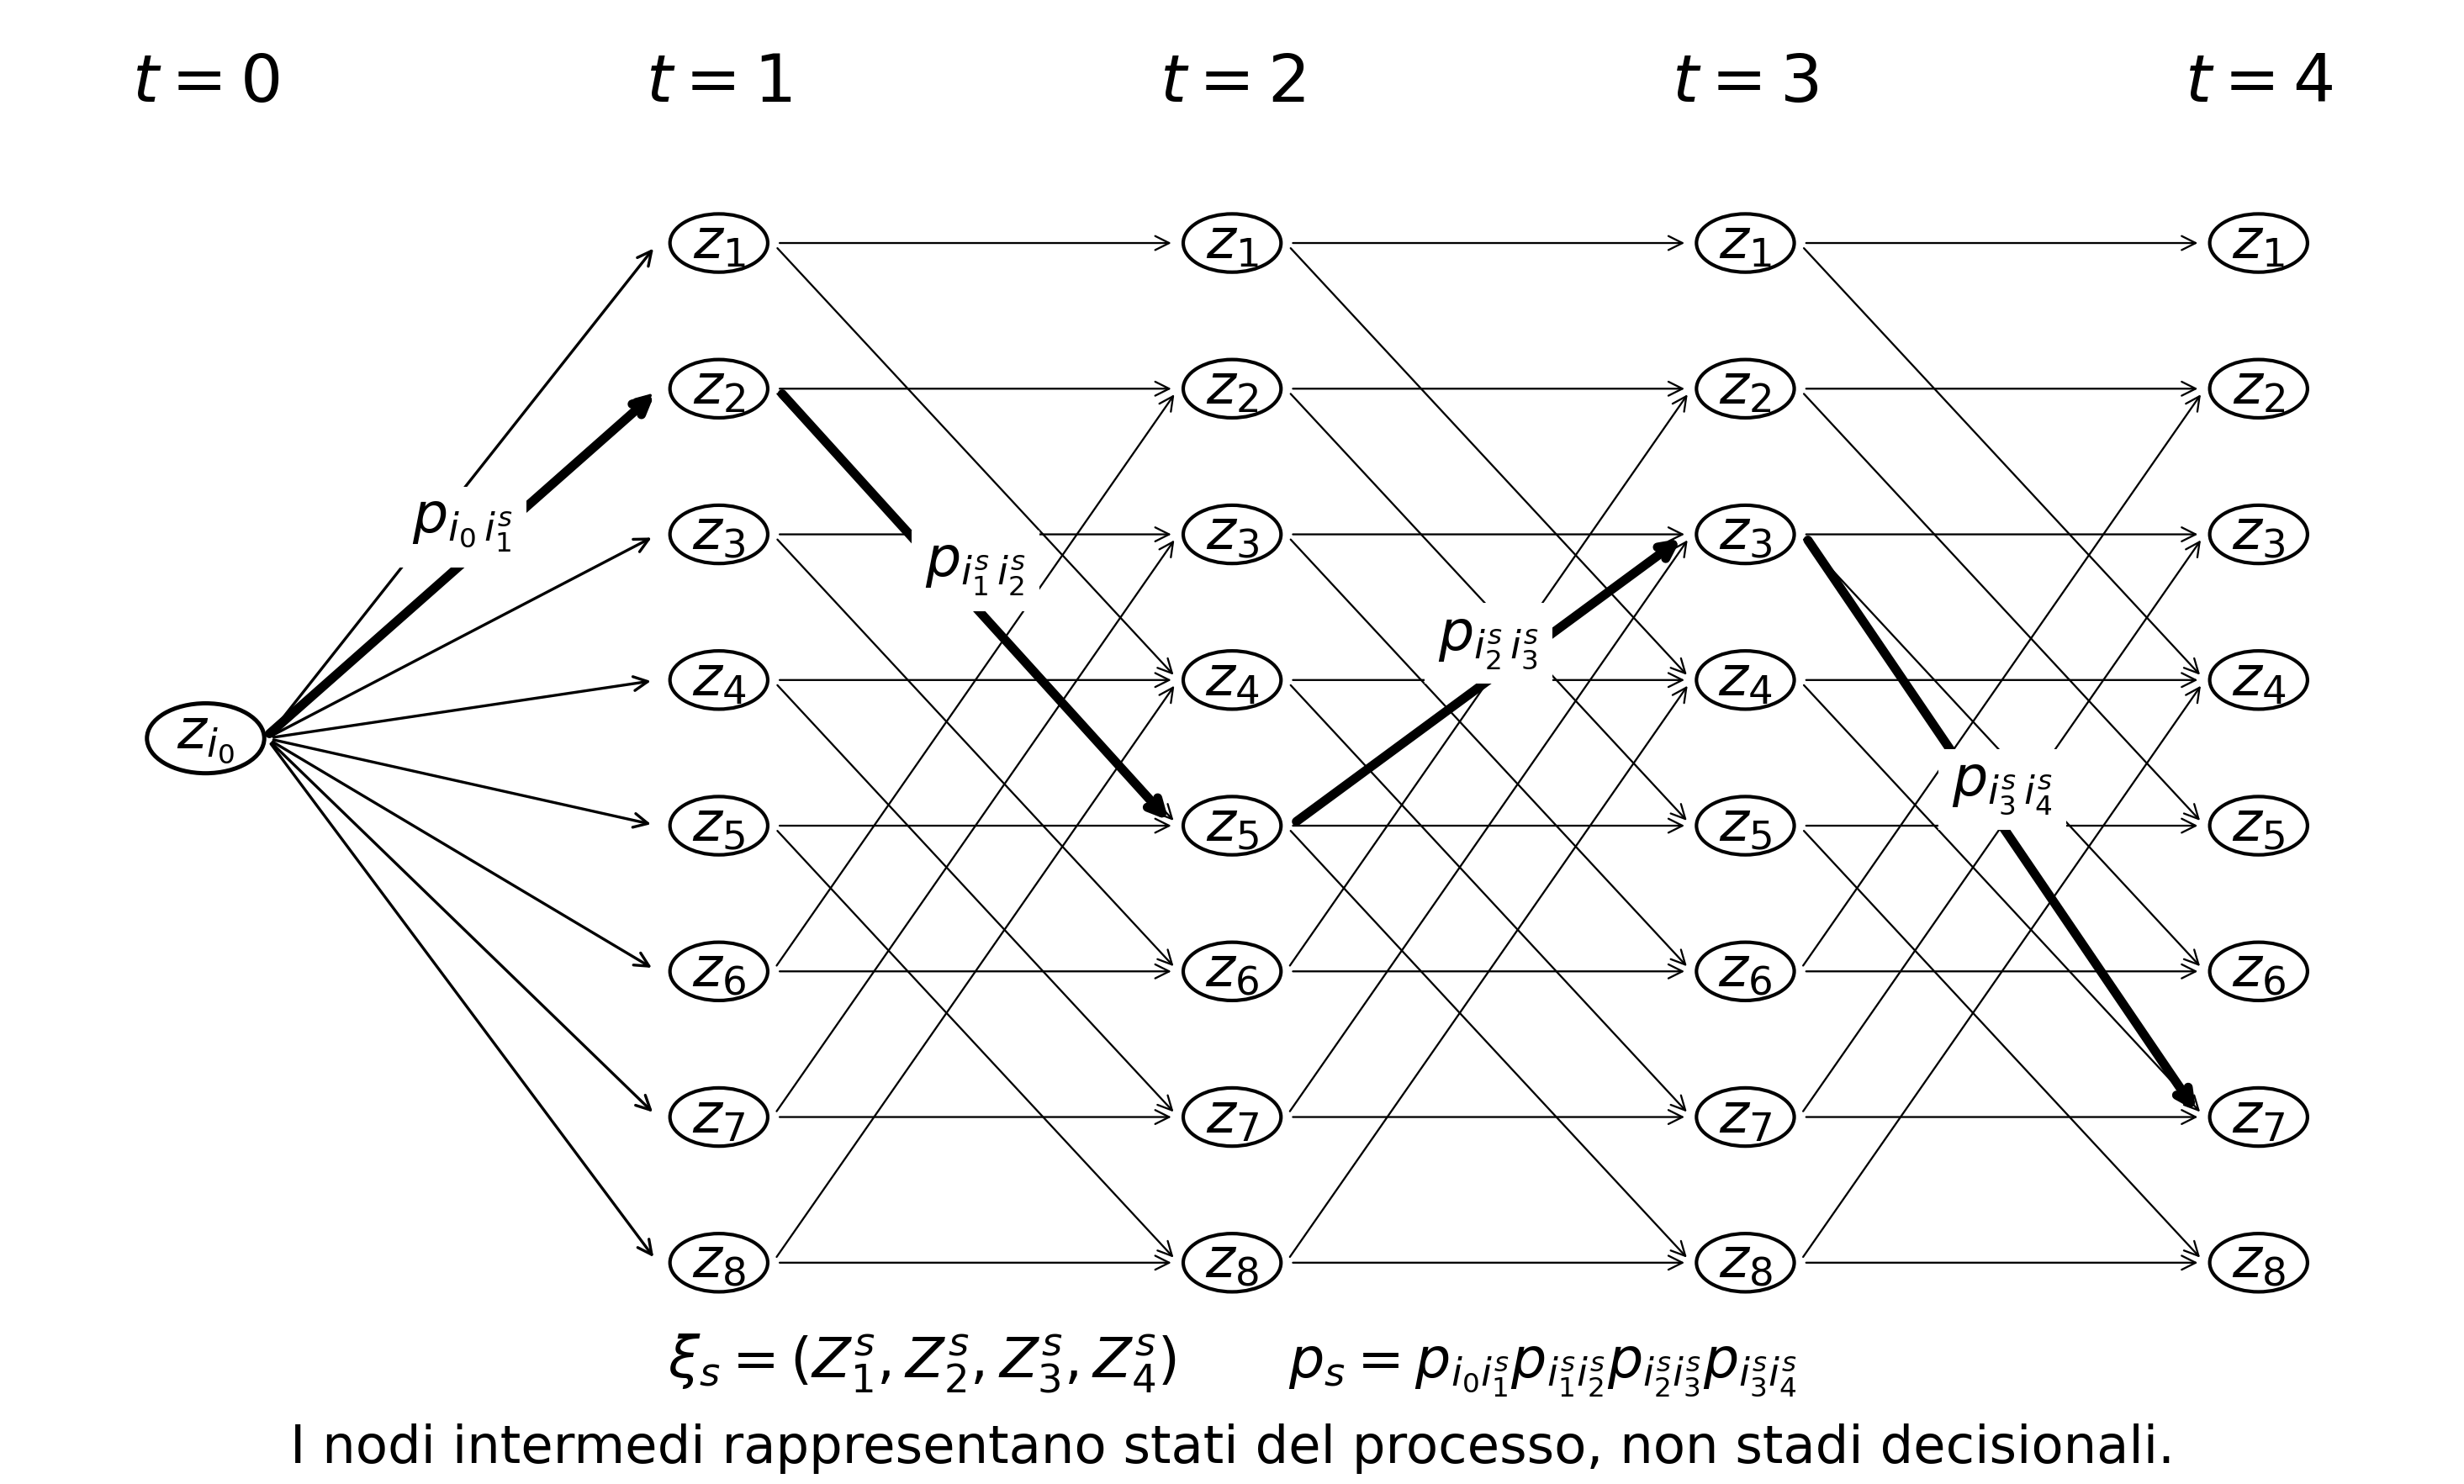
\includegraphics[width=0.72\textwidth]
{../graphics/Cap14_albero_markoviano_scenari.png}
\end{center}

\vspace{-3mm}

Per la propriet\`a di Markov
{\small
\[
p_s=p_{i_0i_1^s}\,p_{i_1^si_2^s}\,p_{i_2^si_3^s}\,p_{i_3^si_4^s},
\qquad
P\longrightarrow\text{traiettorie ammissibili}\longrightarrow\{(\xi_s,p_s)\}.
\]
}

{\footnotesize I nodi intermedi sono stati del processo, non stadi
decisionali: l'intera traiettoria \`e una sola realizzazione osservata prima
del ricorso.}

%TCIMACRO{\TeXButton{Transition: Box Out}{\transboxout}}%
%BeginExpansion
\transboxout%
%EndExpansion
%TCIMACRO{\TeXButton{EndFrame}{\end{frame}}}%
%BeginExpansion
\end{frame}%
%EndExpansion

%****************************************

\subsection{Traiettoria e stato finale}%

%TCIMACRO{\TeXButton{BeginFrame}{\begin{frame}}}%
%BeginExpansion
\begin{frame}%
%EndExpansion

\QTR{frametitle}{Traiettoria o stato finale?}

%TCIMACRO{\TeXButton{Transparency}{\setbeamercovered{transparent=20}}}%
%BeginExpansion
\setbeamercovered{transparent=20}%
%EndExpansion

Dal Capitolo~8, $(P^4)_{i_0j}=\Prob(Z_4=z_j\mid Z_0=z_{i_0})$. Questa
probabilit\`a aggrega tutte le traiettorie che terminano in $z_j$:
\[
(P^4)_{i_0j}=\sum_{s:\;Z_4^s=z_j}p_s.
\]

\begin{stepitemize}
\item La distribuzione terminale \textbf{non} contiene gli stati attraversati
alle date intermedie.

\item Nel caso SVB--ALM quegli stati contano: a ogni data lo stato determina
i coefficienti del modello,
{\small
\[
Z_t^s
\longmapsto
\left(
a_{t1}^s,\ldots,a_{t4}^s,\;
d_t^s,\;
r_t^{g,s},\;
r_t^{u,s},\;
\bar u_t^s
\right).
\]
}
\end{stepitemize}

%TCIMACRO{\TeXButton{Transition: Box Out}{\transboxout}}%
%BeginExpansion
\transboxout%
%EndExpansion
%TCIMACRO{\TeXButton{EndFrame}{\end{frame}}}%
%BeginExpansion
\end{frame}%
%EndExpansion

%****************************************

\section{Esercizio in aula: probabilit\`a di traiettoria e probabilit\`a terminale}

\subsection{La consegna}%

%TCIMACRO{\TeXButton{BeginFrame}{\begin{frame}}}%
%BeginExpansion
\begin{frame}%
%EndExpansion

\QTR{frametitle}{Esercizio: probabilit\`a di traiettoria e probabilit\`a terminale}

%TCIMACRO{\TeXButton{Transparency}{\setbeamercovered{transparent=20}}}%
%BeginExpansion
\setbeamercovered{transparent=20}%
%EndExpansion

{\footnotesize (Capitolo~14, Esercizio svolto~1)}

\medskip

Catena di Markov con stati $\mathcal I=\{z_1,z_2,z_3\}$, stato iniziale
$Z_0=z_1$, orizzonte di due periodi e matrice di transizione
{\small
\[
P=
\begin{pmatrix}
0.7 & 0.2 & 0.1\\
0.1 & 0.6 & 0.3\\
0.2 & 0.3 & 0.5
\end{pmatrix}.
\]
}

\begin{stepenumerate}
\item [1.] Calcolare la probabilit\`a dello scenario $\xi_s=(z_2,z_3)$.

\item [2.] Individuare tutte le traiettorie che terminano nello stato $z_3$
alla data $t=2$ e calcolarne le probabilit\`a.

\item [3.] Determinare $\Prob(Z_2=z_3\mid Z_0=z_1)$ sommando le probabilit\`a
delle traiettorie ottenute al punto precedente.

\item [4.] Verificare il risultato utilizzando la matrice $P^2$ e spiegare la
differenza tra probabilit\`a di una traiettoria e probabilit\`a dello stato
terminale.
\end{stepenumerate}

%TCIMACRO{\TeXButton{Transition: Box Out}{\transboxout}}%
%BeginExpansion
\transboxout%
%EndExpansion
%TCIMACRO{\TeXButton{EndFrame}{\end{frame}}}%
%BeginExpansion
\end{frame}%
%EndExpansion

%****************************************

\subsection{La soluzione}%

%TCIMACRO{\TeXButton{BeginFrame}{\begin{frame}}}%
%BeginExpansion
\begin{frame}%
%EndExpansion

\QTR{frametitle}{Soluzione: una traiettoria e tre traiettorie}

%TCIMACRO{\TeXButton{Transparency}{\setbeamercovered{transparent=20}}}%
%BeginExpansion
\setbeamercovered{transparent=20}%
%EndExpansion

\begin{stepenumerate}
\item [1.] $p_s=p_{12}\,p_{23}=0.2\cdot0.3=0.06$.

\item [2.] $z_1\to z_1\to z_3$: $0.7\cdot0.1=0.07$;
$\;z_1\to z_2\to z_3$: $0.2\cdot0.3=0.06$;
$\;z_1\to z_3\to z_3$: $0.1\cdot0.5=0.05$.

\item [3.] $\Prob(Z_2=z_3\mid Z_0=z_1)=0.07+0.06+0.05=0.18$.

\item [4.] $(P^2)_{13}=0.7(0.1)+0.2(0.3)+0.1(0.5)=0.18$.
\end{stepenumerate}

\medskip

\begin{center}
{\small Una traiettoria ha la sua probabilit\`a $p_s$; lo stato terminale
raccoglie tutte le traiettorie che lo raggiungono.}

\medskip

{\small \textbf{Domanda per la pausa}: fissata $x$ e osservato lo scenario,
che cosa pu\`o ancora fare la banca?}
\end{center}

%TCIMACRO{\TeXButton{Transition: Box Out}{\transboxout}}%
%BeginExpansion
\transboxout%
%EndExpansion
%TCIMACRO{\TeXButton{EndFrame}{\end{frame}}}%
%BeginExpansion
\end{frame}%
%EndExpansion

%****************************************

\section{La funzione di ricorso}

\subsection{Definizione}%

%TCIMACRO{\TeXButton{BeginFrame}{\begin{frame}}}%
%BeginExpansion
\begin{frame}%
%EndExpansion

\QTR{frametitle}{La funzione di ricorso}

%TCIMACRO{\TeXButton{Transparency}{\setbeamercovered{transparent=20}}}%
%BeginExpansion
\setbeamercovered{transparent=20}%
%EndExpansion

Fissati $x$ e $\xi$, la banca risolve ancora un problema di ottimizzazione,
ora deterministico:

\begin{block}{Funzione di ricorso}
{\small
\[
Q(x,\xi)
=
\max_{y\in \mathcal X(\xi)}
\left\{
q(\xi)'y:\;
T(\xi)x+W(\xi)y=h(\xi)
\right\}.
\]
}
\end{block}

{\small
\[
\underbrace{T(\xi)x}_{\text{effetto della decisione iniziale}}
+
\underbrace{W(\xi)y}_{\text{effetto del ricorso}}
=
\underbrace{h(\xi)}_{\text{termine noto}}
\]
}

\begin{stepitemize}
\item $q(\xi)'y$ misura il valore economico del ricorso; $\mathcal X(\xi)$ raccoglie i
vincoli diretti su $y$ (non negativit\`a, limiti operativi).

\item $Q(x,\xi)$ \textbf{non \`e una decisione}: \`e il valore ottimo ottenibile
dopo aver fissato $x$ e osservato $\xi$.
\end{stepitemize}

%TCIMACRO{\TeXButton{Transition: Box Out}{\transboxout}}%
%BeginExpansion
\transboxout%
%EndExpansion
%TCIMACRO{\TeXButton{EndFrame}{\end{frame}}}%
%BeginExpansion
\end{frame}%
%EndExpansion

%****************************************

\subsection{Forma a scenari}%

%TCIMACRO{\TeXButton{BeginFrame}{\begin{frame}}}%
%BeginExpansion
\begin{frame}%
%EndExpansion

\QTR{frametitle}{La funzione di ricorso negli scenari}

%TCIMACRO{\TeXButton{Transparency}{\setbeamercovered{transparent=20}}}%
%BeginExpansion
\setbeamercovered{transparent=20}%
%EndExpansion

{\small
\[
Q_s(x)
=
Q(x,\xi_s)
=
\max_{y_s\in\mathcal X_s}
\left\{
q_s'y_s:\;
T_sx+W_sy_s=h_s
\right\},
\]
\[
q_s=q(\xi_s),
\quad
T_s=T(\xi_s),
\quad
W_s=W(\xi_s),
\quad
h_s=h(\xi_s),
\quad
\mathcal X_s=\mathcal X(\xi_s).
\]
}

\begin{stepitemize}
\item $T_s$ non contiene i vincoli imposti a $x$ quando viene scelta, che
stanno in $\mathcal X_0$: descrive come $x$, ormai fissata, entra nei vincoli
di ricorso dello scenario $s$.

\item Tre oggetti da distinguere:
\begin{itemize}
\item $y_s$, generica decisione di secondo stadio ammissibile;
\item $y_s^*(x)$, decisione ottima di secondo stadio;
\item $Q_s(x)$, valore ottimo prodotto da tale decisione.
\end{itemize}
\end{stepitemize}

%TCIMACRO{\TeXButton{Transition: Box Out}{\transboxout}}%
%BeginExpansion
\transboxout%
%EndExpansion
%TCIMACRO{\TeXButton{EndFrame}{\end{frame}}}%
%BeginExpansion
\end{frame}%
%EndExpansion

%****************************************

\subsection{Coefficienti SVB}%

%TCIMACRO{\TeXButton{BeginFrame}{\begin{frame}}}%
%BeginExpansion
\begin{frame}%
%EndExpansion

\QTR{frametitle}{I coefficienti nel caso SVB--ALM}

%TCIMACRO{\TeXButton{Transparency}{\setbeamercovered{transparent=20}}}%
%BeginExpansion
\setbeamercovered{transparent=20}%
%EndExpansion

{\small $T_s=A^{CF,s}$ raccoglie i cash flow $a_{tj}^s$ (matrice $4\times4$),
$h_s=(d_1^s,\ldots,d_4^s)'$ i fabbisogni,
$y_s=(g_1^s,\ldots,g_4^s,u_1^s,u_2^s,u_3^s)'$ giacenze e funding.}

{\scriptsize
\[
W_s=
\begin{pmatrix}
-1 & 0 & 0 & 0 & 1 & 0 & 0\\
1+r_1^{g,s} & -1 & 0 & 0 & -(1+r_1^{u,s}) & 1 & 0\\
0 & 1+r_2^{g,s} & -1 & 0 & 0 & -(1+r_2^{u,s}) & 1\\
0 & 0 & 1+r_3^{g,s} & -1 & 0 & 0 & -(1+r_3^{u,s})
\end{pmatrix}
\]
}

{\small
\[
q_s=(r_1^{g,s},r_2^{g,s},r_3^{g,s},0,-r_1^{u,s},-r_2^{u,s},-r_3^{u,s})',
\]
\[
\mathcal X_s=\R_+^4\times[0,\bar u_1^s]\times[0,\bar u_2^s]\times[0,\bar u_3^s].
\]
}

\begin{stepitemize}
\item $T_sx+W_sy_s=h_s$ riproduce esattamente i quattro bilanci di liquidit\`a
dello scenario.

\item Nessun nuovo linguaggio: gli stessi coefficienti e vincoli del modello
finanziario del Capitolo~12.
\end{stepitemize}

%TCIMACRO{\TeXButton{Transition: Box Out}{\transboxout}}%
%BeginExpansion
\transboxout%
%EndExpansion
%TCIMACRO{\TeXButton{EndFrame}{\end{frame}}}%
%BeginExpansion
\end{frame}%
%EndExpansion

%****************************************

\section{Esercizio in aula: funzione di ricorso per una decisione assegnata}

\subsection{La consegna}%

%TCIMACRO{\TeXButton{BeginFrame}{\begin{frame}}}%
%BeginExpansion
\begin{frame}%
%EndExpansion

\QTR{frametitle}{Esercizio: funzione di ricorso per una decisione assegnata}

%TCIMACRO{\TeXButton{Transparency}{\setbeamercovered{transparent=20}}}%
%BeginExpansion
\setbeamercovered{transparent=20}%
%EndExpansion

{\footnotesize (Capitolo~14, Esercizio svolto~2)}

\medskip

Un intermediario ha gi\`a assunto $x=(4,\;6)'$. Alla data successiva deve
soddisfare un fabbisogno di liquidit\`a $d=8$; due scenari con $p_1=0.8$ e
$p_2=0.2$.
{\small
\[
a_1'=(1,\;0.8),
\qquad
a_2'=(1,\;0.3),
\qquad
a_s'x+u_s=d+g_s,
\qquad
g_s,u_s\geq0.
\]
}
Costo unitario del funding $1$ nello scenario~1 e $4$ nello scenario~2; la
liquidit\`a residua non produce rendimento.

\medskip

\begin{stepenumerate}
\item [1.] Formulare le due funzioni di ricorso $Q_1(x)$ e $Q_2(x)$.

\item [2.] Determinare le decisioni ottime di secondo stadio nei due scenari.

\item [3.] Calcolare $Q_1(x)$, $Q_2(x)$ e il valore atteso del ricorso.

\item [4.] Se $c'x=x_1+2x_2$, calcolare il valore complessivo della decisione
assegnata.
\end{stepenumerate}

%TCIMACRO{\TeXButton{Transition: Box Out}{\transboxout}}%
%BeginExpansion
\transboxout%
%EndExpansion
%TCIMACRO{\TeXButton{EndFrame}{\end{frame}}}%
%BeginExpansion
\end{frame}%
%EndExpansion

%****************************************

\subsection{La soluzione}%

%TCIMACRO{\TeXButton{BeginFrame}{\begin{frame}}}%
%BeginExpansion
\begin{frame}%
%EndExpansion

\QTR{frametitle}{Soluzione: la stessa decisione vale diversamente}

%TCIMACRO{\TeXButton{Transparency}{\setbeamercovered{transparent=20}}}%
%BeginExpansion
\setbeamercovered{transparent=20}%
%EndExpansion

\begin{stepenumerate}
\item [1.] {\small $Q_1(x)=\max\{-u_1:\;a_1'x+u_1=8+g_1,\ g_1,u_1\geq0\}$,
\newline
$Q_2(x)=\max\{-4u_2:\;a_2'x+u_2=8+g_2,\ g_2,u_2\geq0\}$.}

\item [2.] Scenario~1: $a_1'x=4+0.8\cdot6=8.8$, quindi $u_1^*=0$ e $g_1^*=0.8$.
Scenario~2: $a_2'x=4+0.3\cdot6=5.8$, quindi $u_2^*=2.2$ e $g_2^*=0$.

\item [3.] $Q_1(x)=0$, $\;Q_2(x)=-4\cdot2.2=-8.8$,
$\;\sum_sp_sQ_s(x)=0.8\cdot0+0.2\cdot(-8.8)=-1.76$.

\item [4.] $c'x=4+2\cdot6=16$, quindi
$c'x+\sum_sp_sQ_s(x)=16-1.76=14.24$.
\end{stepenumerate}

\medskip

\begin{center}
{\small Il valore di una decisione iniziale non si legge dal solo $c'x$: la
stessa allocazione produce conseguenze diverse nei diversi scenari.}
\end{center}

%TCIMACRO{\TeXButton{Transition: Box Out}{\transboxout}}%
%BeginExpansion
\transboxout%
%EndExpansion
%TCIMACRO{\TeXButton{EndFrame}{\end{frame}}}%
%BeginExpansion
\end{frame}%
%EndExpansion

%****************************************

\section{Il programma lineare stocastico a due stadi}

\subsection{Definizione}%

%TCIMACRO{\TeXButton{BeginFrame}{\begin{frame}}}%
%BeginExpansion
\begin{frame}%
%EndExpansion

\QTR{frametitle}{Il programma stocastico a due stadi}

%TCIMACRO{\TeXButton{Transparency}{\setbeamercovered{transparent=20}}}%
%BeginExpansion
\setbeamercovered{transparent=20}%
%EndExpansion

\begin{block}{Programma stocastico lineare a due stadi}
{\small
\[
\max_{x\in\mathcal X_0}
\left\{
c'x+\E[Q(x,\xi)]
\right\}
\]
}
\end{block}

\begin{stepitemize}
\item $c'x$ \`e il contributo economico direttamente associato alla decisione
di primo stadio.

\item $\E[Q(x,\xi)]$ \`e il valore atteso della risposta ottimale di secondo
stadio.

\item Per ogni scelta $x$ si considera l'intera distribuzione dei valori di
ricorso, non una sola conseguenza futura.
\end{stepitemize}

\medskip

\[
x
\longrightarrow
Q(x,\xi)
\longrightarrow
\E[Q(x,\xi)]
\]

{\footnotesize La prima freccia \`e l'effetto della decisione iniziale sui
problemi di secondo stadio; la seconda aggrega le conseguenze con la legge di
$\xi$.}

%TCIMACRO{\TeXButton{Transition: Box Out}{\transboxout}}%
%BeginExpansion
\transboxout%
%EndExpansion
%TCIMACRO{\TeXButton{EndFrame}{\end{frame}}}%
%BeginExpansion
\end{frame}%
%EndExpansion

%****************************************

\subsection{Scenari finiti}%

%TCIMACRO{\TeXButton{BeginFrame}{\begin{frame}}}%
%BeginExpansion
\begin{frame}%
%EndExpansion

\QTR{frametitle}{Con un numero finito di scenari}

%TCIMACRO{\TeXButton{Transparency}{\setbeamercovered{transparent=20}}}%
%BeginExpansion
\setbeamercovered{transparent=20}%
%EndExpansion

{\small
\[
\max_{x\in\mathcal X_0}
\Big\{
c'x+\sum_{s\in\mathcal S}p_sQ_s(x)
\Big\}
\]
}

{\small La probabilit\`a $p_s$ non modifica il problema di ricorso dello
scenario $s$: ne pesa il valore ottimo. Esplicitando un ricorso per scenario:}

{\small
\[
\begin{aligned}
\max_{x,\{y_s\}}\quad&
c'x+\sum_{s\in\mathcal S}p_sq_s'y_s\\
\text{s.v.}\quad&
x\in\mathcal X_0,
\qquad
T_sx+W_sy_s=h_s,
\qquad
y_s\in\mathcal X_s,
\qquad
s\in\mathcal S.
\end{aligned}
\]
}

\[
\boxed{
\text{un'unica decisione }x
\quad\text{e}\quad
\text{un ricorso }y_s\text{ per ogni scenario}
}
\]

{\footnotesize Caso SVB--ALM: i quattro bilanci di liquidit\`a vengono
replicati per ogni scenario, mentre il portafoglio iniziale $x$ resta unico.}

%TCIMACRO{\TeXButton{Transition: Box Out}{\transboxout}}%
%BeginExpansion
\transboxout%
%EndExpansion
%TCIMACRO{\TeXButton{EndFrame}{\end{frame}}}%
%BeginExpansion
\end{frame}%
%EndExpansion

%****************************************

\section{Esempio guidato: due scenari}

\subsection{I dati}%

%TCIMACRO{\TeXButton{BeginFrame}{\begin{frame}}}%
%BeginExpansion
\begin{frame}%
%EndExpansion

\QTR{frametitle}{Esempio: allocazione iniziale e funding in due scenari}

%TCIMACRO{\TeXButton{Transparency}{\setbeamercovered{transparent=20}}}%
%BeginExpansion
\setbeamercovered{transparent=20}%
%EndExpansion

{\small $A_0=10$, $x_1+x_2=10$, $x_1,x_2\geq0$; $x_1$ \`e l'attivit\`a pi\`u
liquida, $x_2$ quella pi\`u redditizia: $c'x=x_1+2x_2$. Due scenari,
$p_1=0.75$ e $p_2=0.25$; fabbisogno $d=6$ in entrambi.}

{\small
\[
\text{scenario 1: }\;x_1+0.8x_2+u_1=6+g_1,
\qquad
\text{scenario 2: }\;x_1+0.2x_2+u_2=6+g_2.
\]
}

{\small Costo unitario del funding $1$ e $6$; la liquidit\`a residua non rende.
Dati didattici, non una calibrazione del caso SVB.}

\medskip

\begin{stepitemize}
\item Scenario~1: liquidit\`a $10-0.2x_2\geq8>6$ per ogni $x_2$, quindi
$Q_1(x)=0$.

\item Scenario~2: liquidit\`a $10-0.8x_2$, quindi
\[
Q_2(x)=-6\max\{0,\;0.8x_2-4\}.
\]
Per $x_2\leq5$ la liquidit\`a basta anche nello scenario avverso.
\end{stepitemize}

%TCIMACRO{\TeXButton{Transition: Box Out}{\transboxout}}%
%BeginExpansion
\transboxout%
%EndExpansion
%TCIMACRO{\TeXButton{EndFrame}{\end{frame}}}%
%BeginExpansion
\end{frame}%
%EndExpansion

%****************************************

\subsection{La soluzione}%

%TCIMACRO{\TeXButton{BeginFrame}{\begin{frame}}}%
%BeginExpansion
\begin{frame}%
%EndExpansion

\QTR{frametitle}{La soluzione ottima}

%TCIMACRO{\TeXButton{Transparency}{\setbeamercovered{transparent=20}}}%
%BeginExpansion
\setbeamercovered{transparent=20}%
%EndExpansion

Con $x_1=10-x_2$ il contributo iniziale \`e $10+x_2$ e
\[
V(x_2)=10+x_2-0.25\cdot6\,\max\{0,\;0.8x_2-4\},
\]
\[
V(x_2)=
\begin{cases}
10+x_2, & 0\leq x_2\leq5,\\[2pt]
16-0.2x_2, & 5<x_2\leq10.
\end{cases}
\]

\begin{stepitemize}
\item Fino a $x_2=5$ il valore cresce: pi\`u redditivit\`a, nessun costo di
ricorso.

\item Oltre $x_2=5$ il valore diminuisce: serve funding nello scenario
avverso.

\item Il massimo \`e nel punto di raccordo:
\[
x^*=(5,\;5)',
\qquad
V(x_2^*)=15.
\]
Liquidit\`a $9$ e $6$ nei due scenari: $u_1^*=u_2^*=0$ e
$Q_1(x^*)=Q_2(x^*)=0$.
\end{stepitemize}

%TCIMACRO{\TeXButton{Transition: Box Out}{\transboxout}}%
%BeginExpansion
\transboxout%
%EndExpansion
%TCIMACRO{\TeXButton{EndFrame}{\end{frame}}}%
%BeginExpansion
\end{frame}%
%EndExpansion

%****************************************

\subsection{Il confronto}%

%TCIMACRO{\TeXButton{BeginFrame}{\begin{frame}}}%
%BeginExpansion
\begin{frame}%
%EndExpansion

\QTR{frametitle}{Perch\'e non tutto nell'attivo pi\`u redditizio}

%TCIMACRO{\TeXButton{Transparency}{\setbeamercovered{transparent=20}}}%
%BeginExpansion
\setbeamercovered{transparent=20}%
%EndExpansion

{\small
\renewcommand{\arraystretch}{1.25}
\begin{center}
\begin{tabular}{c|c|c|c}
\hline
decisione & $c'x$ & $\sum_sp_sQ_s(x)$ & $c'x+\sum_sp_sQ_s(x)$\\
\hline
$(0,\;10)'$ & $20$ & $-6$ & $14$\\
$(5,\;5)'$ & $15$ & $0$ & $15$\\
\hline
\end{tabular}
\end{center}
}

\medskip

\begin{stepitemize}
\item L'allocazione concentrata ha il risultato di primo stadio pi\`u alto, ma
il costo atteso del ricorso ne riduce il valore complessivo.

\item L'allocazione bilanciata \textbf{non} \`e imposta da un vincolo di
prudenza: emerge dall'ottimizzazione.

\item Oltre $x_2=5$ il beneficio marginale della redditivit\`a \`e pi\`u che
compensato dal costo atteso del funding nello scenario avverso.
\end{stepitemize}

\medskip

\begin{center}
{\small La decisione iniziale si sceglie considerando come modifica le
possibilit\`a e i costi di reazione nei diversi scenari.}
\end{center}

%TCIMACRO{\TeXButton{Transition: Box Out}{\transboxout}}%
%BeginExpansion
\transboxout%
%EndExpansion
%TCIMACRO{\TeXButton{EndFrame}{\end{frame}}}%
%BeginExpansion
\end{frame}%
%EndExpansion

%****************************************

\section{Forma estesa e non anticipativit\`a}

\subsection{Definizione}%

%TCIMACRO{\TeXButton{BeginFrame}{\begin{frame}}}%
%BeginExpansion
\begin{frame}%
%EndExpansion

\QTR{frametitle}{La forma estesa}

%TCIMACRO{\TeXButton{Transparency}{\setbeamercovered{transparent=20}}}%
%BeginExpansion
\setbeamercovered{transparent=20}%
%EndExpansion

I due livelli si riuniscono in un unico programma lineare deterministico,
con una copia delle variabili di ricorso per ciascuno scenario:

\begin{block}{Forma estesa}
{\small
\[
\begin{aligned}
\max_{x,\{y_s\}_{s\in\mathcal S}}\quad&
c'x+\sum_{s\in\mathcal S}p_sq_s'y_s\\
\text{soggetto a}\quad&
x\in\mathcal X_0,\\
&T_sx+W_sy_s=h_s,
\qquad s\in\mathcal S,\\
&y_s\in\mathcal X_s,
\qquad s\in\mathcal S.
\end{aligned}
\]
}
\end{block}

\begin{stepitemize}
\item \`E un programma lineare deterministico di dimensione maggiore.

\item L'incertezza non compare pi\`u come variabile casuale: \`e rappresentata
dalla presenza simultanea di tutti gli scenari e dei loro pesi.
\end{stepitemize}

%TCIMACRO{\TeXButton{Transition: Box Out}{\transboxout}}%
%BeginExpansion
\transboxout%
%EndExpansion
%TCIMACRO{\TeXButton{EndFrame}{\end{frame}}}%
%BeginExpansion
\end{frame}%
%EndExpansion

%****************************************

\subsection{Struttura a blocchi}%

%TCIMACRO{\TeXButton{BeginFrame}{\begin{frame}}}%
%BeginExpansion
\begin{frame}%
%EndExpansion

\QTR{frametitle}{Struttura a blocchi}

%TCIMACRO{\TeXButton{Transparency}{\setbeamercovered{transparent=20}}}%
%BeginExpansion
\setbeamercovered{transparent=20}%
%EndExpansion

{\small Con tre scenari i vincoli di secondo stadio sono}
{\small
\[
\begin{pmatrix}
T_1 & W_1 & 0 & 0\\
T_2 & 0 & W_2 & 0\\
T_3 & 0 & 0 & W_3
\end{pmatrix}
\begin{pmatrix}
x\\
y_1\\
y_2\\
y_3
\end{pmatrix}
=
\begin{pmatrix}
h_1\\
h_2\\
h_3
\end{pmatrix}.
\]
}

\begin{stepitemize}
\item La decisione di primo stadio $x$ compare in \textbf{tutti} i blocchi di
scenario.

\item Ciascun vettore di ricorso $y_s$ compare \textbf{soltanto} nei vincoli
del proprio scenario.

\item Dimensione: con $n_x$ variabili di primo stadio, $n_y$ variabili e $m_y$
vincoli di ricorso per scenario, la forma estesa ha $n_x+|\mathcal S|\,n_y$
variabili e $|\mathcal S|\,m_y$ vincoli di secondo stadio. Il numero di
scenari diventa centrale.
\end{stepitemize}

%TCIMACRO{\TeXButton{Transition: Box Out}{\transboxout}}%
%BeginExpansion
\transboxout%
%EndExpansion
%TCIMACRO{\TeXButton{EndFrame}{\end{frame}}}%
%BeginExpansion
\end{frame}%
%EndExpansion

%****************************************

\subsection{Non anticipativita}%

%TCIMACRO{\TeXButton{BeginFrame}{\begin{frame}}}%
%BeginExpansion
\begin{frame}%
%EndExpansion

\QTR{frametitle}{Non anticipativit\`a}

%TCIMACRO{\TeXButton{Transparency}{\setbeamercovered{transparent=20}}}%
%BeginExpansion
\setbeamercovered{transparent=20}%
%EndExpansion

\begin{block}{Non anticipativit\`a}
{\small Una decisione soddisfa il principio di non anticipativit\`a se
dipende soltanto dall'informazione disponibile nel momento in cui viene
assunta.}
\end{block}

\medskip

\[
\boxed{
x\text{ \`e unico e comune a tutti gli scenari,}
\qquad
y_s\text{ dipende dallo scenario }s.}
\]

\begin{stepitemize}
\item Decisioni di primo stadio distinte per scenario,
$x_1,\ldots,x_{|\mathcal S|}$, attribuirebbero indebitamente al decisore la
conoscenza anticipata del futuro.

\item Con un unico vettore $x$ la non anticipativit\`a \`e incorporata nella
forma estesa: non servono vincoli aggiuntivi.

\item Vincoli espliciti servono quando si introducono copie scenario-specifiche
della stessa decisione.
\end{stepitemize}

%TCIMACRO{\TeXButton{Transition: Box Out}{\transboxout}}%
%BeginExpansion
\transboxout%
%EndExpansion
%TCIMACRO{\TeXButton{EndFrame}{\end{frame}}}%
%BeginExpansion
\end{frame}%
%EndExpansion

%****************************************

\section{Esercizio in aula: forma estesa e non anticipativit\`a}

\subsection{La consegna}%

%TCIMACRO{\TeXButton{BeginFrame}{\begin{frame}}}%
%BeginExpansion
\begin{frame}%
%EndExpansion

\QTR{frametitle}{Esercizio: forma estesa e non anticipativit\`a}

%TCIMACRO{\TeXButton{Transparency}{\setbeamercovered{transparent=20}}}%
%BeginExpansion
\setbeamercovered{transparent=20}%
%EndExpansion

{\footnotesize (Capitolo~14, Esercizio svolto~3)}

\medskip

{\small Due scenari con $p_1=0.6$ e $p_2=0.4$. Decisione iniziale
$x=(x_1,x_2)'$ con $x_1+x_2=10$, $x_1,x_2\geq0$; contributo
$c'x=x_1+1.5x_2$. Ricorso $y_s=(g_s,u_s)'$ con $g_s,u_s\geq0$ e bilanci}
{\small
\[
x_1+0.9x_2+u_1=7+g_1,
\qquad
x_1+0.4x_2+u_2=7+g_2.
\]
}
{\small Costo unitario del funding $1$ nel primo scenario e $3$ nel secondo.}

\medskip

\begin{stepenumerate}
\item [1.] Scrivere la forma estesa del programma stocastico.

\item [2.] Individuare quali variabili sono comuni ai due scenari e quali sono
scenario-specifiche.

\item [3.] Spiegare perch\'e una formulazione con due decisioni iniziali
indipendenti $x^{(1)}$ e $x^{(2)}$ non rappresenterebbe correttamente il
problema a due stadi.

\item [4.] Mostrare come sarebbe possibile utilizzare copie scenario-specifiche
della decisione iniziale mantenendo la non anticipativit\`a.
\end{stepenumerate}

%TCIMACRO{\TeXButton{Transition: Box Out}{\transboxout}}%
%BeginExpansion
\transboxout%
%EndExpansion
%TCIMACRO{\TeXButton{EndFrame}{\end{frame}}}%
%BeginExpansion
\end{frame}%
%EndExpansion

%****************************************

\subsection{La soluzione}%

%TCIMACRO{\TeXButton{BeginFrame}{\begin{frame}}}%
%BeginExpansion
\begin{frame}%
%EndExpansion

\QTR{frametitle}{Soluzione: una decisione iniziale, due ricorsi}

%TCIMACRO{\TeXButton{Transparency}{\setbeamercovered{transparent=20}}}%
%BeginExpansion
\setbeamercovered{transparent=20}%
%EndExpansion

\begin{stepenumerate}
\item [1.] Forma estesa:
{\small
\[
\begin{array}{ll}
\max & x_1+1.5x_2-0.6u_1-1.2u_2\\[2pt]
\text{s.v.} & x_1+x_2=10,\\
& x_1+0.9x_2+u_1-g_1=7,\qquad x_1+0.4x_2+u_2-g_2=7,\\
& x_1,x_2,g_1,g_2,u_1,u_2\geq0.
\end{array}
\]
}

\item [2.] $x_1,x_2$ sono comuni ai due scenari; $(g_1,u_1)$ appartengono solo
allo scenario~1, $(g_2,u_2)$ solo allo scenario~2.

\item [3.] Con $x^{(1)}$ e $x^{(2)}$ indipendenti il modello sceglierebbe
l'allocazione iniziale in base allo scenario che si realizzer\`a: userebbe al
primo stadio un'informazione disponibile solo al secondo.

\item [4.] Le copie sono ammesse se si impone $x^{(1)}=x^{(2)}$; pi\`u
semplicemente si usa un unico vettore $x$.
\end{stepenumerate}

%TCIMACRO{\TeXButton{Transition: Box Out}{\transboxout}}%
%BeginExpansion
\transboxout%
%EndExpansion
%TCIMACRO{\TeXButton{EndFrame}{\end{frame}}}%
%BeginExpansion
\end{frame}%
%EndExpansion

%****************************************

\section{Sintesi}

\subsection{Il percorso}%

%TCIMACRO{\TeXButton{BeginFrame}{\begin{frame}}}%
%BeginExpansion
\begin{frame}%
%EndExpansion

\QTR{frametitle}{Il percorso della lezione}

%TCIMACRO{\TeXButton{Transparency}{\setbeamercovered{transparent=20}}}%
%BeginExpansion
\setbeamercovered{transparent=20}%
%EndExpansion

\[
\boxed{
\text{un unico futuro noto}
\qquad\longrightarrow\qquad
\text{pi\`u futuri possibili}
}
\]

\medskip

{\small
\[
\begin{aligned}
&\text{modello probabilistico}
\longrightarrow
\text{scenari}
\longrightarrow
\text{ricorso}\\
&\hspace{2.0cm}
\longrightarrow
\text{programma stocastico}
\longrightarrow
\text{forma estesa}
\end{aligned}
\]
}

\medskip

\begin{stepitemize}
\item La funzione obiettivo combina il \textbf{valore della decisione
iniziale} e il \textbf{valore atteso del ricorso}.

\item Non si cerca pi\`u un piano ottimo per un futuro considerato noto, ma una
decisione iniziale che tenga conto delle diverse evoluzioni possibili e delle
azioni correttive successive.
\end{stepitemize}

%TCIMACRO{\TeXButton{Transition: Box Out}{\transboxout}}%
%BeginExpansion
\transboxout%
%EndExpansion
%TCIMACRO{\TeXButton{EndFrame}{\end{frame}}}%
%BeginExpansion
\end{frame}%
%EndExpansion

%****************************************

\subsection{Sintesi}%

%TCIMACRO{\TeXButton{BeginFrame}{\begin{frame}}}%
%BeginExpansion
\begin{frame}%
%EndExpansion

\QTR{frametitle}{Che cosa portiamo a casa}

%TCIMACRO{\TeXButton{Transparency}{\setbeamercovered{transparent=20}}}%
%BeginExpansion
\setbeamercovered{transparent=20}%
%EndExpansion

\begin{stepenumerate}
\item [1.] \textbf{Stadi e periodi} sono concetti distinti: un problema
multiperiodale pu\`o avere due soli stadi decisionali.

\item [2.] Uno \textbf{scenario} \`e una traiettoria completa con la sua
probabilit\`a; da una catena di Markov $p_s$ \`e il prodotto delle
transizioni.

\item [3.] $Q_s(x)$ \`e il \textbf{valore della migliore risposta} disponibile
dopo aver fissato $x$ e osservato lo scenario.

\item [4.] La \textbf{forma estesa} ha un'unica $x$ e un ricorso $y_s$ per
scenario: \`e qui che la non anticipativit\`a diventa visibile.
\end{stepenumerate}

\medskip

\begin{center}
{\small \textbf{Lezione~15}: quando il ricorso esiste, come dipende da $x$ e
quanto vale la soluzione stocastica.}
\end{center}

%TCIMACRO{\TeXButton{Transition: Box Out}{\transboxout}}%
%BeginExpansion
\transboxout%
%EndExpansion
%TCIMACRO{\TeXButton{EndFrame}{\end{frame}}}%
%BeginExpansion
\end{frame}%
%EndExpansion

%****************************************

\end{document}
